\section{CoFaaS}
% Following the previous section, we now begin to see how we can use Wasm components to reduce the communication latency of FaaS application in a language-independent fashion.

% Since Wasm components are conceptually similar to FaaS functions and likewise facilitate composition, at a high level, we need two things to use Wasm components to reduce the communication latency of FaaS applications. We need to \begin{inparaenum}[1)] \item compile the target FaaS function to Wasm and \item transform the original IDL specification of the FaaS function to WIT as used by the Wasm component model.
%   \end{inparaenum}

In this section, we discuss the design and implementation details of CoFaaS and describe how a FaaS function is transformed. We start by describing how the IDL mapping is performed, then we introduce the concept of a CoFaaS \emph{component} and finally we discuss the combined transformation workflow.

\begin{figure}
  \centering
  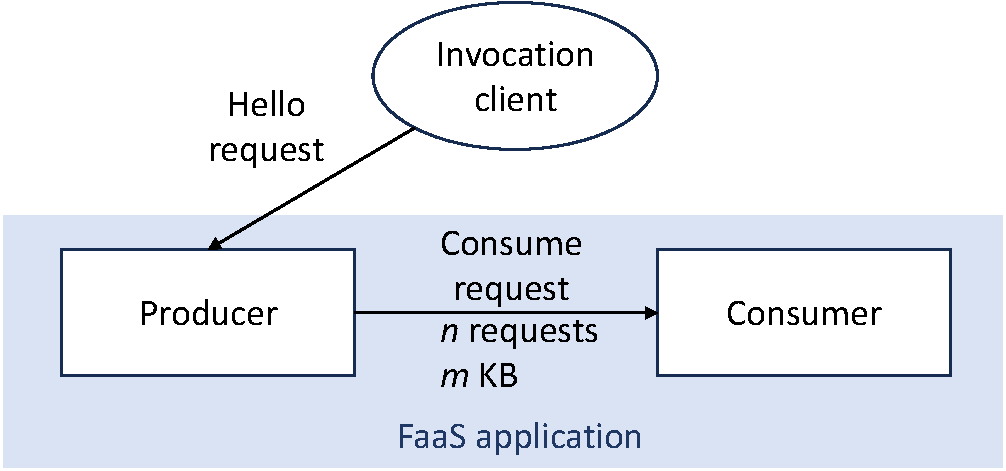
\includegraphics[width=\columnwidth]{figures/experimental_setup}
  \caption{\label{fig:func-setup} Schematic of the FaaS application used for evaluating CoFaaS}
\end{figure}

To describe CoFaaS functionality, we will use a simple two-function FaaS application, named Prodcon, that we will also revisit in the evaluation section (\Cref{sec:evaluation}). The application is shown in \Cref{fig:func-setup}. The functionality of this application is simple: when the Producer function receives a request from the Invocation Client it sends one or more requests to the Consumer function. The size of the request can be varied and it does not need to have any particular structure.

% 2 pages

% - Describe how each function is transformed into a composable Wasm component


\subsection{IDL mapping}
\label{subsec:idl-mapping}

\begin{sidewaysfigure}
  \centering
  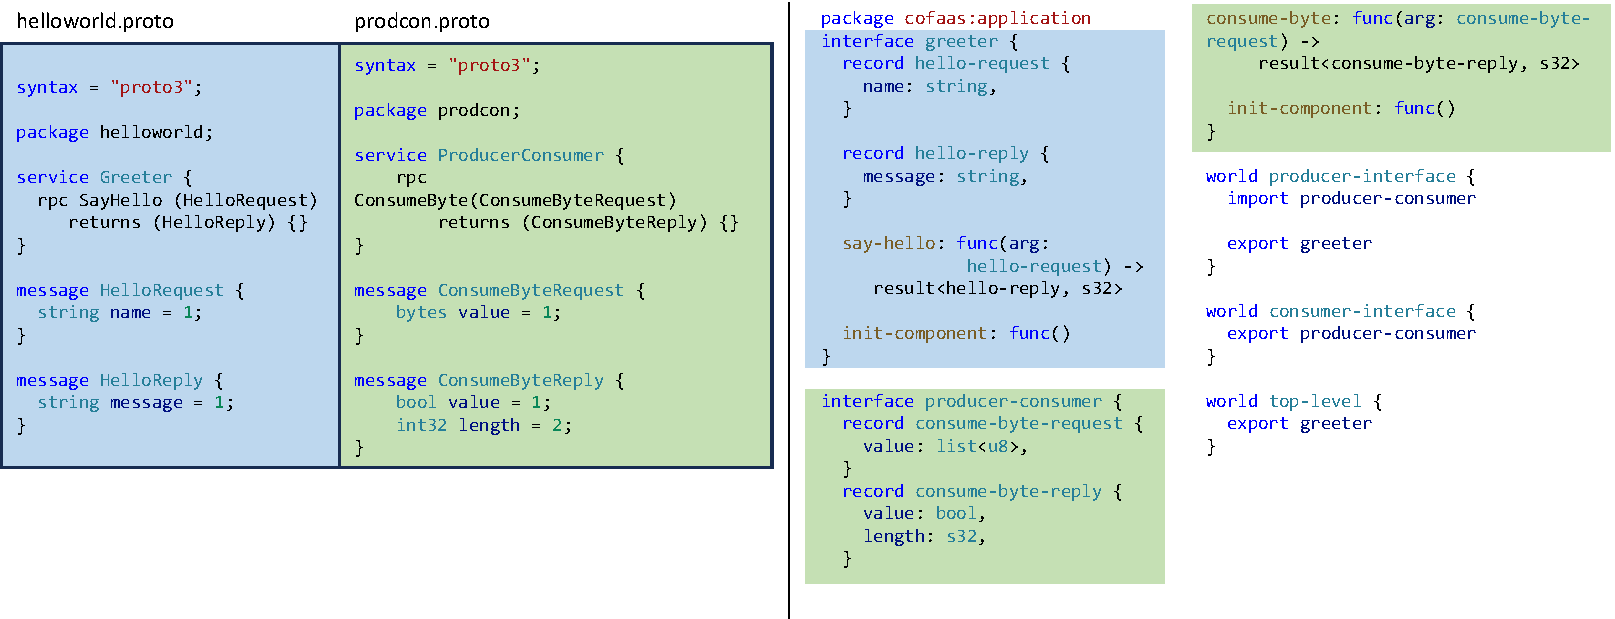
\includegraphics[width=\textwidth]{figures/idf_transformation}
  \caption{\label{fig:wit-transformation} Example showing how gRPC (left) is transformed to the Wasm Interface Type (WIT) (right).}
\end{sidewaysfigure}
% I moved the figures around to make the labels match the flow of the text (Fig 4 was previously discussed before Fig 3)

As mentioned in introduction, a FaaS function must have a contract that specifies how it interacts with the surrounding world. For this purpose, it is common to use Interface Definition Languages that formally defines a function's inputs and output. An IDL is purely declarative, a key reason for their language-independence, and therefore they rely on code generators to be turned into a usable interface.

In practice, several different IDLs are in use by real-world FaaS applications, two notable examples being Protobuf~\cite{protobuf}, used by Google's gRPC~\cite{grpc}, and Apache Thrift~\cite{thrift}. Currently, CoFaaS only supports gRPC but there is no fundamental limitation preventing other IDLs from being supported. In the following, we will detail how the transformation from Protobuf to Wasm's WIT is done.

\Cref{fig:wit-transformation} shows an example of how two gRPC interfaces, marked by the blue and green shades respectively, are transformed into their equivalent WIT definitions. Referring to the Prodcon application of \Cref{fig:func-setup}, the Producer function \emph{exports} the \texttt{helloworld} protocol and \emph{imports} the \texttt{prodcon} protocol. The Consumer function only exports the \texttt{prodcon} protocol. The interfaces exported by a function can be called by other functions whereas the interfaces imported by a function can be used to call another function exporting the same interface.

We will start by describing the structure of the \texttt{prodcon} gRPC interface. The interface consists of two \emph{messages} and one \emph{service}. In gRPC terms, a message is equivalent to a \texttt{struct} in C. For example, looking at the \texttt{prodcon} protocol in \Cref{fig:wit-transformation} we see that it defines two messages: \texttt{ConsumeByte}-\texttt{Request} and \texttt{ConsumeByteResponse}. Additionally, it defines a single service \texttt{ProducerConsumer} that defines a single method named \texttt{ConsumeByte}. To put this in the terminology of a conventional program, a function exporting the \texttt{prodcon} interface will expose a public API containing the \texttt{ConsumeByte} function that takes a struct of type \texttt{Consume}-\texttt{ByteRequest} as an argument and returns a struct of type \texttt{ConsumeByteReply}.

%Now that we understand the left side of \Cref{fig:wit-transformation} and how it relates to the application shown in \Cref{fig:func-setup}, 
Next, we describe how the WIT interface on the right is generated. As an input to the process, the developer currently needs to add a metadata file to each FaaS function that specifies the import and export protocols of the function. This is not strictly necessary and can be easily replaced by a static code analysis step that infers this information. The WIT generator takes all of the protocols used by functions in the applications and does the following: \begin{inparaenum}[a)] \item it maps each protocol to a WIT \emph{interface} and \item it generates a WIT \emph{world} for each function in the application. Further, it generates a world called \texttt{top-level} that defines the public interface of the whole application. \end{inparaenum} A WIT world represents the entire public interface of a function, as such, we see that the world corresponding to the producer function, \texttt{producer-interface}, imports the \texttt{producer-consumer} interface enabling the Producer function is able to call the Consumer function. It exports the \texttt{greeter} interface as this is the external interface of the application.

For each interface generated the WIT notion of a \texttt{record} corresponds to a \texttt{message} in gRPC and services are represented as a sequence of function definitions. We also note the addition of a \texttt{init-component} function. This method calls the \texttt{main} method of the original FaaS functions to perform necessary initialization of the function. When a CoFaaS-transformed application is loaded, all of its comprising functions chain-calls their \texttt{init-component} methods.

\subsection{FaaS Function to CoFaaS Component}
\label{subsec:cofaascomp}

\begin{figure}
  \centering
  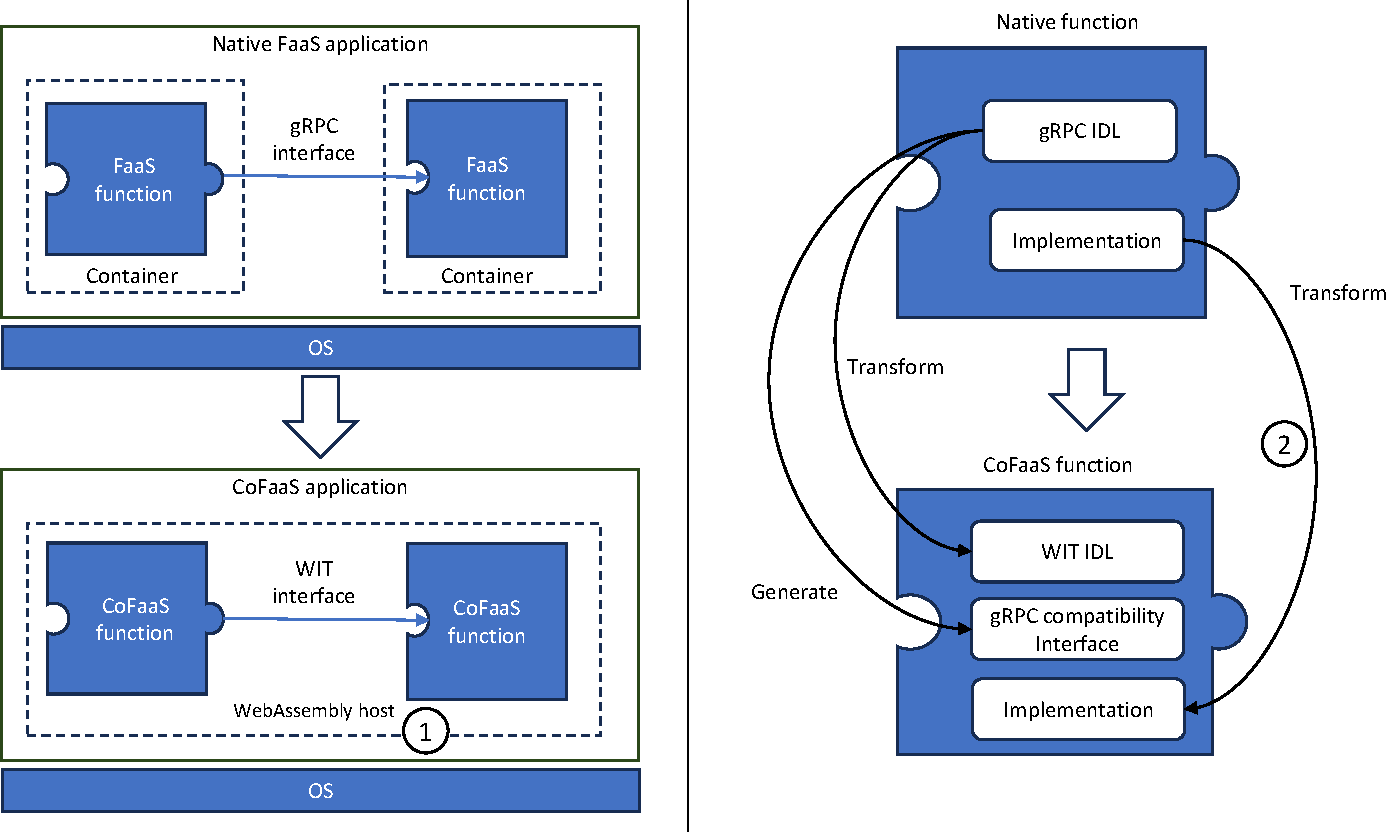
\includegraphics[width=\textwidth]{figures/components_overview}
  \caption{\label{fig:cofaas-transformation} Overview of the CoFaaS transformation process. }
\end{figure}

In the FaaS computing model, functions are the fundamental building block that applications are composed of. The CoFaaS transformation takes each FaaS function and transforms it into a different, but analogous, building block known as a CoFaaS component. In this section, we describe how a FaaS function is turned into a CoFaaS component and how CoFaaS components can be recomposed into different application in the same way as FaaS functions. An overview of the transformation process is given in \Cref{fig:cofaas-transformation}. The left side of the figure shows the high-level overview of the CoFaaS transformation, particularly how the inter-function communication interface is transformed and how the functions are changed from running in a separate container to sharing a runtime on the same WebAssembly host. The right side of the function shows how the individual functions are transformed. The functions are represented as puzzle pieces to emphasize their composability. In the rest of this section, we will refer to the circled numbers in the figure to explain each step.

% The previous section focused on one particular aspect of this transformation, namely how to turn a gRPC interface into a WIT interface. much more goes into the creation of a CoFaaS component.

Generating a CoFaaS component is equivalent to a separate compilation step.  A standard FaaS function contains code compiled to a binary that is then packed in a container that is brought up on nodes as needed. When generating a CoFaaS component, the compilation step is preceded by CoFaaS code generators and code transformers. The resulting code is then compiled to a CoFaaS component. Crucially, this step can be performed ahead-of-time in a similar way as a normal FaaS function is turned into a container. Once the CoFaaS components are built, generating a CoFaaS application by composing components is fast, and can be done on the fly on a host at deployment time. We revisit this in \Cref{subsec:practice}.

Next, we describe how the implementation code of the original function is transformed \textcircled{2}. To ensure that we preserve the semantics of the original functions, CoFaaS seeks to change the implementation code of the original functions as little as possible. However, since the original code of the FaaS functions 1) expects to run as a separate server process that listens to a network request and 2) use the API generated by the gRPC code generator for communicating with the outside world, we can not entirely avoid minor changes to the application code.

The default code generator for gRPC produces code that uses networked RPC calls for communicating with other functions. When transforming a FaaS function to a CoFaaS component, we need to eliminate and replace this RPC-backed communication. At the same time, since we want to avoid changing the original implementation code as much as possible, we also need to maintain compatibility with the API produced by the gRPC code generator. To achieve this, we implement a custom gRPC code generator that generates code conforming to the same API as the gRPC-generated code but replaces network-backed RPC calls with local function calls. Additionally, the interface code that we generate contains a small wrapper that translates between the data structures passed from the Wasm component call and the gRPC-defined data structures that are used by the implementation code.

%Now, there is only one part left of our function transformation journey: dealing
Finally, we need to deal 
with redundant library calls. For example, a function using gRPC for communication uses the following code for initializing a connection to a server.
\begin{minted}{go}
conn, err := grpc.Dial(addr, grpc.WithBlock(), [...])
[...]
client := pb_client.NewProducerConsumerClient(conn)
\end{minted}
The resulting \texttt{client} object holds a interface that can be used to communicate with the Consumer process in \Cref{fig:func-setup}. The first call to \texttt{grpc.Dial} initializes a network connection that is used as the transport for the RPC call. In our case, initialing this networking connection is not needed. Now, recall again that we want to avoid modifying the original implementation code as much as possible. Therefore, rewriting the implementation code to remove the call to \texttt{grpc.Dial} is not an option. To handle this, we therefore introduce our own stubbed gRPC library replacement that provides a simple \texttt{nop} implementation of the \texttt{Dial} function defined as follows
\begin{minted}{go}
func Dial(target string, opts ...interface{})
         (*ClientConn, error) {
    return &ClientConn{}, nil
}
\end{minted}

This library stubbing technique allows us to change the behavior of the function without directly transforming critical parts of its code. If we performed such transformation automatically, it would be difficult to ensure that we do not break the behavior of existing code in the process. At the same time, we avoid executing redundant and/or undesired operations present in the original code. Making the rewritten code use our stubbed library is simple: we simply change the gRPC import of the client code to use our library instead. We also provide a stubbed version of the built-in Go \texttt{net} library.

Currently, we always replace imports of these libraries with our stubbed versions. For cases where all gRPC calls are transformed to local CoFaaS calls this works well. However, this is not always desirable. Functions may want to open network connections for other reasons. To support this, it is trivial to add a code analysis step to the code transformation that determines which libraries specific gRPC calls are related to and only replace libraries that are related to the gRPC calls that we want to turn into local CoFaaS calls.

The final step involved is to generate the Wasm host wrapper \textcircled{1} that hosts a Wasm runtime and will load and run the CoFaaS application. This host wrapper exposes a gRPC interface corresponding to the public interface of the FaaS application. When requests are received by this wrapper, they are transformed into a call to the WIT bindings of the first function of the CoFaaS application.

\subsection{Putting it all together}
\label{subsec:cofaas-overview}

In summary, following are the steps for applying the CoFaaS transformation to a FaaS application. We emphasize that all of these steps are completely automated.

\begin{enumerate}
\item The WIT code generator is invoked to transform the gRPC protocols used by the FaaS functions to a WIT interface describing the entire application \Cref{subsec:idl-mapping}
\item For every FaaS function, we generate bindings for its corresponding WIT world and use our custom gRPC code generators to generate a compatibility layer between the gRPC API used by the function implementation and the WIT bindings used for communicating within the CoFaaS application
\item Then, we apply a set of transformations to the implementation code of the function. These transformations make the code use the replacement gRPC API that we generate and make the code use our stub libraries to disable undesired functionality
  \item  Finally, we generate the Wasm host wrapper that exposes the external interface of the FaaS application over gRPC and loads and runs the CoFaaS application.
\end{enumerate}

To add support for a new language in CoFaaS, only steps 2 and 3 above need to be re-implemented. Steps 1 and 4 are generic and doesn't change regardless of the function implementation language. Current, CoFaaS supports applying this transformation to functions written in Go automatically. For Rust, we manually rewrite function code in a way that is identical to the automated process.

\subsection{CoFaaS in Practice}
\label{subsec:practice}

\begin{figure}
  \centering
  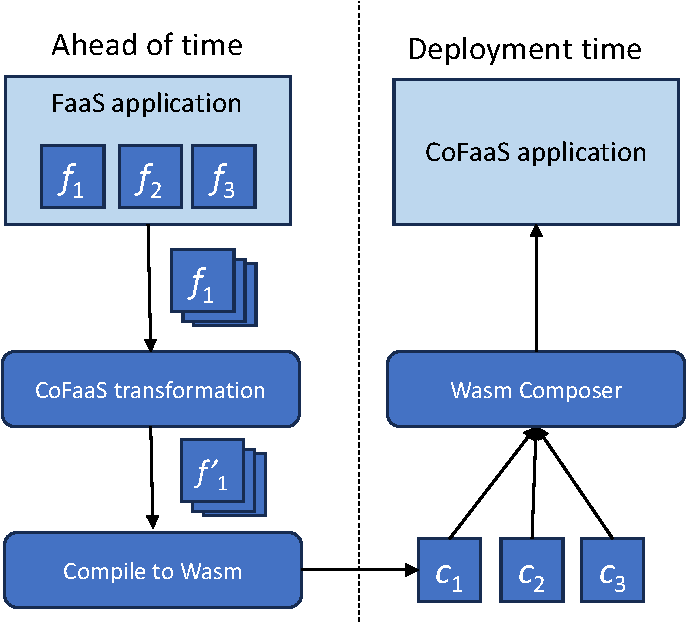
\includegraphics[width=\columnwidth]{figures/cofaas_compilation}
  \caption{\label{fig:compile} The workflow of applying the CoFaaS transformation to a FaaS application.}
\end{figure}

As previously mentioned, applying the CoFaaS transformation to a FaaS application involves several steps. Some of these can be can be done of time as part of application development and packaging while others can be performed at deployment time. The workflow is depicted in \Cref{fig:compile}. The first step is to take the functions comprising a FaaS application and apply the CoFaaS transformation to them. The mechanics of this transformation is described earlier in this section. The output of the CoFaaS transformation is the source code needed to create a CoFaaS component. By compiling the transformed functions to Wasm we turn them into CoFaaS components, labeled $c{1..3}$ in the figure. The final step is to feed the CoFaaS component through the Wasm compositor that yields the resulting CoFaaS application, a single Wasm binary containing the entire application. An important detail here is that the ``Ahead of time'' steps are, like compilation, potentially quite time consuming. The ``Deployment time'' composition step, on the other hand, is fast and can be performed instantaneously. This means that we can re-use CoFaaS components in several applications by dynamically re-composing them on deployment. In this way, CoFaaS maintains the flexibility of native FaaS deployments.

% [at runtime, however, CoFaaS differs from a standard container implementation. Normal orchestration by bringing containers up, in CoFaaS, orchestration by composing components. This yields a monolith application and is therefore less ``agile'' but the composition is quick and is faster than bringing up and moving around normal containers]


% \subsection{Overheads}
% \label{subsec:overheads}

%%% Local Variables:
%%% mode: latex
%%% TeX-master: "main"
%%% TeX-command-extra-options: "-shell-escape"
%%% End:
